% ----------------------------------------------------------------------
% Configurar a classe do documento
% ----------------------------------------------------------------------
\documentclass[12pt]{article}

% ----------------------------------------------------------------------
% Definir packages externos, língua, margens, tipos de letra, novos 
% comandos e cores
% ----------------------------------------------------------------------
\usepackage[utf8]{inputenc} % Codificação utilizada
\usepackage[english]{babel} % Idioma de escrita

\usepackage[export]{adjustbox} % Alinhar imagens
\usepackage{amsmath} % Comandos extra para escrita matemática
\usepackage{amssymb} % Símbolos matemáticos
\usepackage{anysize} % Personalizar as margens
    \marginsize{2cm}{2cm}{2cm}{2cm} % {esquerda}{direita}{cima}{baixo}
\usepackage{appendix} % Apêndices
\usepackage{cancel} % Cancelar expressões
\usepackage{caption} % Legendas
    \DeclareCaptionFont{newfont}{\fontfamily{cmss}\selectfont}
    \captionsetup{labelfont={bf, newfont}}
\usepackage{cite} % Citações, tipo [1 - 3]
\usepackage{color} % Colorir texto
\usepackage{fancyhdr} % Cabeçalho e rodapé
    \pagestyle{fancy}
    \fancyhf{}
    \fancyhead[L]{\footnotesize\fontfamily{cmss}\selectfont IST} % Esquerda do cabeçalho
    \fancyhead[R]{\footnotesize\fontfamily{cmss}\selectfont ULisboa} % Direita do cabeçalho
    \fancyfoot[L]{\footnotesize\fontfamily{cmss}\selectfont Robotics} % Esquerda do rodapé
    \fancyfoot[C]{\thepage} % Centro do rodapé
    \fancyfoot[R]{\footnotesize\fontfamily{cmss}\selectfont MEEC} % Direita do rodapé
    \renewcommand{\footrulewidth}{0.4pt} % Régua do rodapé
\usepackage{float} % Utilizar o especificador [H] nas figuras
\usepackage{graphicx} % Imagens em LaTeX
\usepackage[colorlinks = true, plainpages = true, linkcolor = istblue, urlcolor = istblue, citecolor = istblue, anchorcolor = istblue]{hyperref}
\usepackage{indentfirst} % Primeiro parágrafo
\usepackage{siunitx} % Unidades SI
\usepackage{subcaption} % Subfiguras
\usepackage{titlesec} % Tipo de letra
    \titleformat{\section}{\fontfamily{cmss}\selectfont\Large\bfseries}{\thesection}{1em}{}
    \titleformat{\subsection}{\fontfamily{cmss}\selectfont\large\bfseries}{\thesubsection}{1em}{}
    \titleformat{\subsubsection}{\fontfamily{cmss}\selectfont\normalsize\bfseries}{\thesubsubsection}{1em}{}
    \fancyfoot[C]{\fontfamily{cmss}\selectfont\thepage}

% Encher de texto aleatório (apagar)
\usepackage{lipsum}
\usepackage{duckuments}

% Novos e renovar comandos
\newcommand{\sen}{\operatorname{\sen}} % Definição da função seno
\newcommand{\HRule}{\rule{\linewidth}{0.5mm}} % Definição de uma régua
\renewcommand{\appendixpagename}{\LARGE \fontfamily{cmss}\selectfont Appendices}
\renewcommand{\appendixtocname}{Appendices}

% Cores
\definecolor{istblue}{RGB}{3, 171, 230}
\definecolor{dkgreen}{rgb}{0,0.6,0}
\definecolor{gray}{rgb}{0.5,0.5,0.5}

%%%%%%%%%%%%%%%%%%%%%%%%%%%%%%%%%%%%%%%%%%%%%%%%%%%%%%%%%%%%%%%%%%%%%%%%
%                               Documento                              %
%%%%%%%%%%%%%%%%%%%%%%%%%%%%%%%%%%%%%%%%%%%%%%%%%%%%%%%%%%%%%%%%%%%%%%%%
\begin{document}

% ----------------------------------------------------------------------
% Capa
% ----------------------------------------------------------------------
\begin{center}
    \begin{figure}
        \vspace{-1.0cm}
        
\includegraphics[scale = 0.3, left]{Imagens/IST_A.eps} % Tipo de assinatura do IST
    \end{figure}
    \mbox{}\\[2.0cm]
    \textsc{\Huge Robotics}\\[2.5cm]
    \textsc{\LARGE MEEC}\\[2.0cm]
    \HRule\\[0.4cm]
    {\large \bf {\fontfamily{cmss}\selectfont Orientation Estimation and Trajectory Analysis Using Sensor Data}}\\[0.2cm]
    \HRule\\[1.5cm]
\end{center}

\begin{flushleft}
    \textbf{\fontfamily{cmss}\selectfont Authors:}
\end{flushleft}

\begin{center}
    \begin{minipage}{0.5\textwidth}
        \begin{flushleft}
            Vladimiro José de Medeiros Roque (98589)\\
            José Pedro da Cunha Rodrigues (113234)\\
            Miguel Rodrigues Ferreira (113289)\\
            Pedro Alexandre Ferreira Dias Lopes (103194)
        \end{flushleft}
    \end{minipage}%
    \begin{minipage}{0.5\textwidth}
        \begin{flushright}
            \href{mailto:vladimiro.roque@tecnico.ulisboa.pt}{\texttt{vladimiro.roque@tecnico.ulisboa.pt}}\\
            \href{mailto:jose.p.rodrigues@tecnico.ulisboa.pt}{\texttt{jose.p.rodrigues@tecnico.ulisboa.pt}}\\
            \href{mailto:miguel.r.ferreira@tecnico.ulisboa.pt}{\texttt{miguel.r.ferreira@tecnico.ulisboa.pt}}
            \href{mailto:pedroafdlopes@tecnico.ulisboa.pt}{\texttt{pedroafdlopes@tecnico.ulisboa.pt}}
        \end{flushright}
    \end{minipage}
\end{center}
    
\begin{flushleft}
    \large $\boxed{\text{\bf \fontfamily{cmss}\selectfont Group} \ \textbf{9}}$\\[4.0cm]
\end{flushleft}
    
\begin{center}
    \large \bf \fontfamily{cmss}\selectfont 2024/2025 -- 1º Semester, P2
\end{center}

\thispagestyle{empty}

\setcounter{page}{0}

\newpage

% ----------------------------------------------------------------------
% Conteúdo
% ----------------------------------------------------------------------
\tableofcontents 

\newpage

% ----------------------------------------------------------------------
% Desenvolvimento
% ----------------------------------------------------------------------
\section{Group Members Contribution} % Professor pediu esta seção, está nos slides da teorica (1º slides)

\section{Introduction} 

This laboratory assignment focuses on two core objectives: understanding the estimation of orientation using data from a rate-gyro sensor and an accelerometer, and demonstrating the application of an industrial-grade serial manipulator. By addressing these objectives, students will gain practical experience in processing sensor data, applying mathematical models, and reconstructing trajectories in both Cartesian and orientation spaces.
The work begins with the analysis of sensor data, provided in unique datasets for each group, containing approximately 20 seconds of measurements. The initial 5 seconds represent a static phase where the sensor remains stationary, providing a baseline for filtering and processing. These datasets include accelerometer readings (in milli-g) and rate-gyro readings (in degrees per second), formatted to facilitate computational analysis.
The assignment is divided into multiple tasks, starting with data visualization, filtering, and theoretical trajectory reconstruction equations. Further tasks involve the graphical representation of reconstructed trajectories and their interpretation. In the later stages, the focus shifts to the use of the Scorbot VII manipulator. Here, students will derive the robot's direct kinematics equations and assess whether the reconstructed trajectories can be executed by the manipulator.
By combining theoretical concepts with practical implementation, this lab offers an in-depth understanding of sensor data processing and robotic manipulator operations. 

\newpage

\section{Tasks}

\subsection{Task 1}

Task 1 involves visualizing sensor data by plotting the components of the accelerometer and rate-gyro measurements along their respective axes. This step is critical for understanding the behavior of the sensor during the data collection process and identifying any initial patterns or anomalies in the raw data.
The dataset provided contains time-stamped measurements from an accelerometer and a rate-gyro, with values distributed across three axes: x, y, and z. The accelerometer data (measured in milli-g) reflects linear acceleration along each axis, while the rate-gyro data (measured in degrees per second) provides angular velocity along the same axes. The first few seconds of the dataset capture the sensor in a static configuration, offering a baseline for comparison against later movements.
Through the visualization of these components in a combined plot, we aim to:

\begin{itemize}
    \item Distinguish the data trends for each axis.
    \item Identify any irregularities or noise in the data.
    \item Provide a foundation for further processing in subsequent tasks.
    \item This initial analysis will serve as the starting point for understanding the sensor's performance and the nature of the motion captured.
\end{itemize}


\begin{figure}[H]
    \centerline{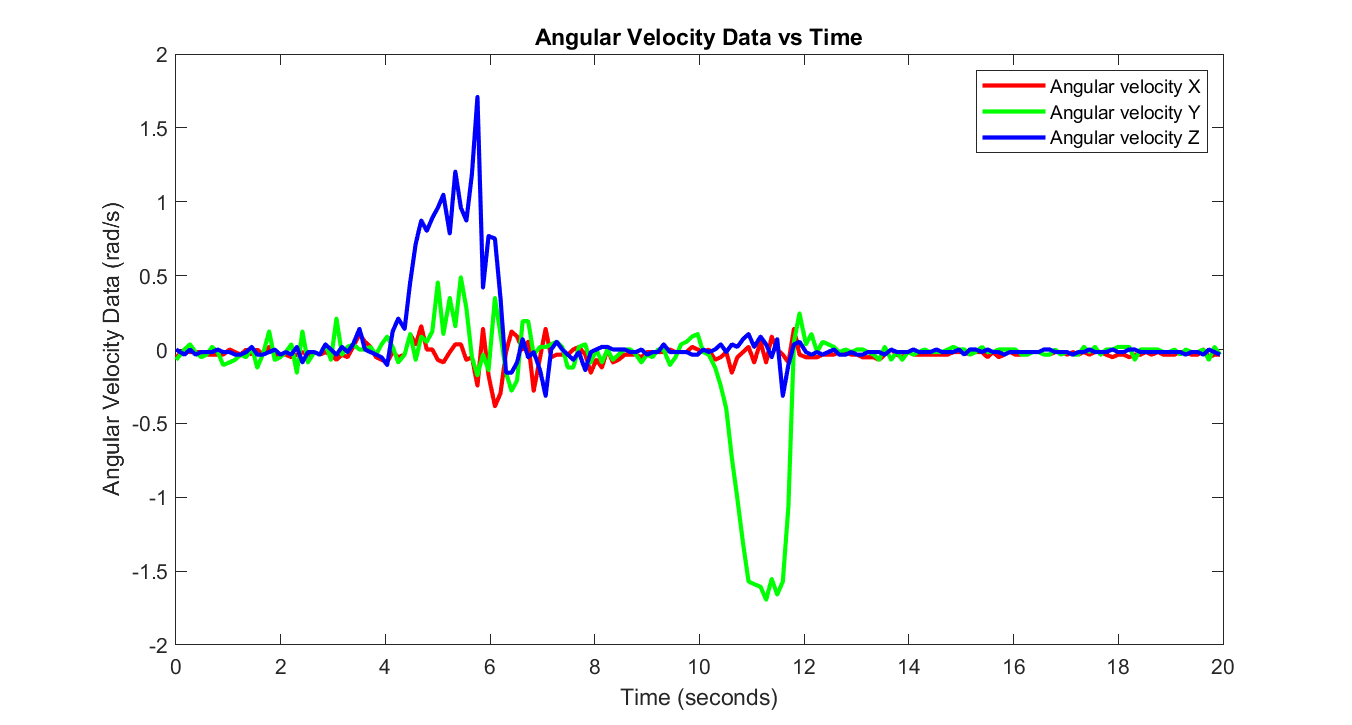
\includegraphics[scale=0.7]{Imagens/angularvstime.png}}
    \caption{Angular velocity vs time.}
    \label{fig}
\end{figure}


\begin{figure}[H]
    \centerline{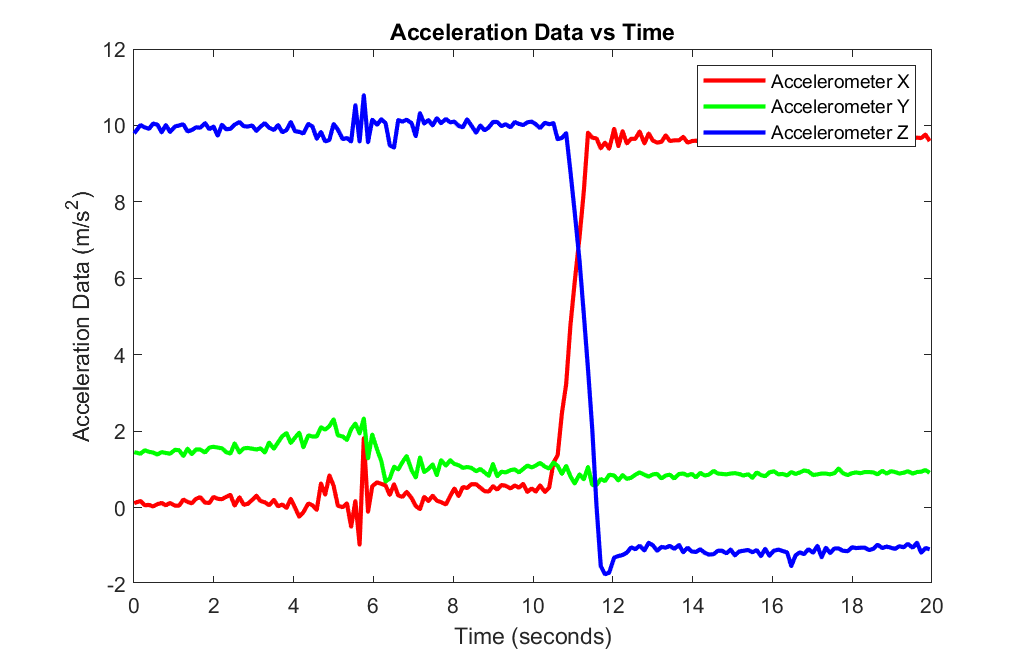
\includegraphics[scale=0.7]{Imagens/acclerationvstime.png}}
    \caption{Acceleration vs time}
    \label{fig}
\end{figure}

\subsection*{Z-Axis (Blue Line)}

In the acceleration graph, the blue line starts near \(10 \, \mathrm{m/s^2}\), which corresponds to the gravitational acceleration. This confirms that the blue line represents the \(z\)-axis, as it aligns with gravity during the static phase of the robotic arm.

In the angular velocity graph, the blue line represents \(\omega_z\) (angular velocity around the \(z\)-axis). As expected, there is a strong correlation between the changes in acceleration and angular velocity along this axis:
\begin{itemize}
    \item For example, at around 12 seconds, both acceleration and angular velocity show a significant negative dip, confirming the \(z\)-axis mapping.
\end{itemize}

\subsection*{X-Axis (Red Line)}

In the acceleration graph, the red line shows values near \(0 \, \mathrm{m/s^2}\) during the static phase, confirming that it is not aligned with gravity. However, during the dynamic phase (after \(\sim 5\) seconds), it shows significant positive and negative variations due to movement along this axis.

In the angular velocity graph, the red line represents \(\omega_x\) (angular velocity around the \(x\)-axis). We observe that:
\begin{itemize}
    \item When the angular velocity (\(\omega_x\)) increases positively (e.g., around 6 seconds), the corresponding acceleration (\(a_x\)) also shows a positive variation.
    \item This synchronized behavior validates that the red lines in both graphs represent the \(x\)-axis.
\end{itemize}

\subsection*{Y-Axis (Green Line)}

In the acceleration graph, the green line remains near a low positive value during the static phase, indicating that it is neither aligned with gravity nor orthogonal to it. During the dynamic phase, it exhibits moderate oscillations due to translational and rotational effects.

In the angular velocity graph, the green line represents \(\omega_y\) (angular velocity around the \(y\)-axis). Observing the dynamic phase:
\begin{itemize}
    \item Positive peaks in \(\omega_y\) (e.g., around 6 seconds) correspond to similar positive peaks in \(a_y\), confirming the mapping of the green line to the \(y\)-axis.
\end{itemize}

\subsection*{Alignment in Variation}

For all three axes (\(x\), \(y\), and \(z\)), we observe that when the angular velocity increases positively, the corresponding acceleration also increases positively. Similarly, when the angular velocity decreases or becomes negative, the corresponding acceleration exhibits a similar negative variation. This consistent relationship occurs because:

\subsubsection*{Rotational Dynamics Influence Linear Dynamics}
\begin{itemize}
    \item In a robotic arm, each joint's motion generates a combination of tangential and centripetal accelerations, which are directly tied to the angular velocity and its rate of change.
    \item The tangential acceleration depends on the rate of change of angular velocity (\(\dot{\omega}\)), while the centripetal acceleration depends on the square of angular velocity (\(\omega^2\)) and acts perpendicular to the direction of rotation.
\end{itemize}

\subsubsection*{Controlled System Dynamics}
\begin{itemize}
    \item Robotic arms are designed for precise and coordinated movements. Each joint is controlled by motors that apply predictable torques, resulting in synchronized changes in angular velocity and acceleration.
    \item When a joint rotates positively (e.g., \(\omega_x > 0\)), it induces a linear acceleration along the same axis as part of the controlled rotational motion.
\end{itemize}

\subsubsection*{Fixed Axis of Rotation}
\begin{itemize}
    \item Unlike free-moving objects, the axes of rotation in a robotic arm are fixed, ensuring that the measured angular velocities and accelerations align in their respective directions without interference from external or random forces.
\end{itemize}

This predictable alignment between angular velocity and acceleration highlights the consistency of the robotic arm's motion and validates the observed variations in the provided graphs.



\subsection{Task 2}

Preprocessing sensor data is a vital step to ensure accurate and meaningful analysis. Raw data, collected from accelerometers and rate-gyros, often contain noise and occasional outliers caused by sensor imperfections, environmental factors, or abrupt movements. These irregularities can obscure the true motion dynamics and negatively affect subsequent analyses.
In this case, a median filter was applied to clean the data effectively. This filtering technique is well-suited for handling outliers and reducing noise, as it replaces each data point with the median of its neighbors within a defined window. Unlike other filtering methods, the median filter preserves sharp transitions and edges in the data while removing unwanted spikes, making it ideal for dynamic motion data.
The results achieved with the median filter demonstrated significant improvements, yielding smooth and reliable datasets without distortions. This preprocessing ensures that the data is well-prepared for reconstructing accurate trajectories and performing further analysis with confidence in the validity of the underlying patterns.

\begin{figure}[H]
    \centerline{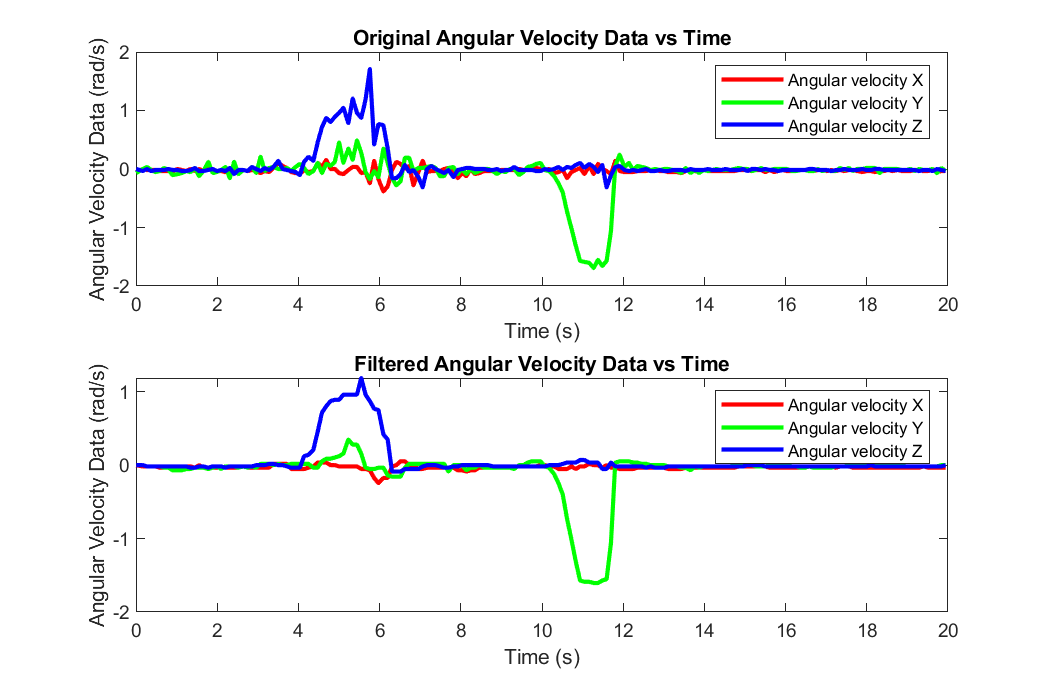
\includegraphics[scale=0.8]{Imagens/filteredangularvsoriginal.png}}
    \caption{Filtered angular velocity vs original (using median filter).}
    \label{fig}
\end{figure}


\begin{figure}[H]
    \centerline{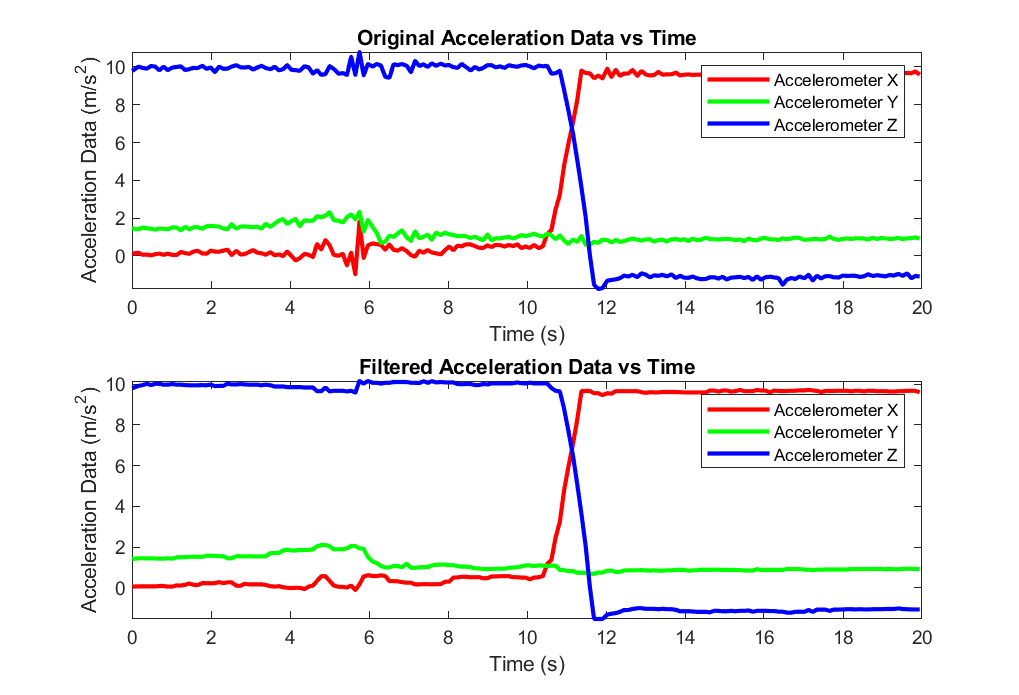
\includegraphics[scale=0.8]{Imagens/filteredaccelerationvsoriginal.png}}
    \caption{Filtered acceleration vs original (using median filter)}
    \label{fig}
\end{figure}


\subsection*{Comparison of Filters}

\paragraph{1. Sliding Window Average/Median Filters}
\begin{itemize}
    \item \textbf{Average Filter:} 
    Calculates the average of data points within a sliding window, effectively reducing high-frequency noise. However, it is sensitive to outliers, as extreme values can significantly skew the average.
    \item \textbf{Median Filter:} 
    Replaces each point with the median of its neighbors within the sliding window. This makes it more robust than the average filter, as it can effectively handle outliers without distorting the signal.
\end{itemize}

\paragraph{2. Gaussian Filters}
\begin{itemize}
    \item Smooths data by applying a weighted average, where weights follow a Gaussian distribution. This reduces noise while preserving overall trends better than simple averaging.
    \item It is less robust to outliers compared to the median filter, as the weights are still influenced by extreme values.
    \item Requires the selection of a standard deviation parameter (\(\sigma\)), which controls the level of smoothing, making it less straightforward for general applications.
\end{itemize}

\paragraph{3. Savitzky–Golay Filters}
\begin{itemize}
    \item Fits a polynomial to a subset of data points within a sliding window, then replaces the center point with the value predicted by the polynomial.
    \item Effective at preserving sharp transitions and trends while reducing noise, making it ideal for smooth but non-linear signals.
    \item Sensitive to outliers, as the polynomial fit can be distorted by extreme values within the window.
    \item Requires careful tuning of the polynomial order and window size for optimal results.
\end{itemize}

\paragraph{4. Smooth Filters}
\begin{itemize}
    \item General-purpose filters that reduce noise by averaging data points or applying weighted smoothing.
    \item These filters can smooth data effectively but often blur sharp transitions, making them less suitable for dynamic systems like robotic arms.
    \item They do not specifically address outliers, which can still influence the smoothed result.
\end{itemize}

\paragraph{5. Outliers Filters}
\begin{itemize}
    \item Specifically designed to detect and remove outliers based on statistical thresholds (e.g., Z-Score or Interquartile Range methods).
    \item While effective at identifying and removing anomalies, these filters often leave gaps in the data by replacing outliers with \texttt{NaN}, requiring additional interpolation steps.
    \item Do not inherently smooth the data or reduce noise in non-outlier regions.
\end{itemize}

\subsection*{Why Use the Median Filter?}
The Median Filter stands out compared to these alternatives due to its:
\begin{itemize}
    \item \textbf{Robustness:} Unlike the Average, Gaussian, or Savitzky–Golay filters, the Median Filter is highly robust against outliers and extreme values, as it is unaffected by the magnitude of data points outside the sliding window.
    \item \textbf{Preservation of Trends:} The Median Filter preserves sharp transitions and dynamic changes better than smooth or Gaussian filters, which tend to over-smooth the data.
    \item \textbf{Simplicity:} Requires only a window size as a parameter, making it simpler to implement than Gaussian or Savitzky–Golay filters, which require tuning of additional parameters (e.g., \(\sigma\) or polynomial order).
    \item \textbf{Completeness:} Unlike Outliers Filters, the Median Filter does not leave gaps in the data and simultaneously reduces noise and removes anomalies.
\end{itemize}


\subsection{Task 3}


To reconstruct the sensor position in Cartesian coordinates  \(({x}, {y}, {z})\) using accelerometer data, we analyze the relationship between acceleration data \((\ddot{x}, \ddot{y}, \ddot{z}\)) and the velocity data we get from integrating the acceleration \((\dot{x}, \dot{y}, \dot{z}\)) . 


\subsubsection{Theory and Mathematical Formulation}

\begin{itemize}
    \item \textbf{X} — Position on the global x axis.  
    \item \textbf{Y} — Position on the global y axis.
    \item \textbf{Z} — Position on the global z axis.
\end{itemize}

\paragraph{Parameterization}

To reconstruct the position accurately, we define the following parameters:
\begin{itemize}
    \item \( x, y, z \): Position components in the Cartesian space.
    \item \(\dot{x},\dot{y},\dot{z}\): Velocity components, which are the first derivatives of position (first derivatives).
    \item \(\ddot{x},\ddot{y},\ddot{z}\): Acceleration components, which are the second derivatives of position (second derivatives).
    \item \(\Delta{t}\): Sampling period of the acceleration data. 
\end{itemize} 

\subsubsection{Effect of Gravity}

The acceleration due to gravity must be taken into account when reconstructing the sensor position in the Cartesian coordinates. The gravitational acceleration is approximated as \( g = 9.8 \, \text{m/s}^2 \) in the downward direction along the global z-axis. The total acceleration vector in the world frame, \( \mathbf{A} \), is the final accelerations only due to the motion of the sensor.

The equation for the total acceleration vector is:

\[
\mathbf{A} = \mathbf{R} \cdot \begin{bmatrix} \ddot{x} \\ \ddot{y} \\ \ddot{z} \end{bmatrix} - 9.8 \cdot \begin{bmatrix} 0 \\ 0 \\ 1 \end{bmatrix}
\]

Where:
- \( \mathbf{R} \) is the transformation matrix, calculated in \textbf{Orientation Representation}, that relates the accelerometer's local frame to the world frame.
- \( \ddot{x}, \ddot{y}, \ddot{z} \) are the accelerations along the x, y, and z axes, respectively.
- The second term \( -9.8 \cdot \begin{bmatrix} 0 \\ 0 \\ 1 \end{bmatrix} \) represents the gravitational acceleration in the world frame.

This equation allows us to separate the accelerometer’s linear motion from the gravitational effect, enabling a more accurate reconstruction of the sensor's position.




\section*{Position and Velocity Update}

\subsection*{General Formulas}

In general, the position update equations for discrete system can be written as:
\[
\mathbf{p}(t + \Delta t) = \mathbf{p}(t) + \mathbf{v}(t) \Delta t + \frac{1}{2} \mathbf{a}(t) (\Delta t)^2
\]

The velocity update equation is:
\[
\mathbf{v}(t + \Delta t) = \mathbf{v}(t) + \mathbf{a}(t) \Delta t
\]

\subsection*{Matrix Notation for \(x, y, z\) Components}

Using matrix notation, the updates become:

\[
\begin{bmatrix} x(t+ \Delta t) \\ y(t+ \Delta t) \\ z(t+ \Delta t) \end{bmatrix}
= 
\begin{bmatrix} x(t) \\ y(t) \\ z(t) \end{bmatrix}
+ 
\begin{bmatrix} \dot{x}(t) \\ \dot{y}(t) \\ \dot{z}(t) \end{bmatrix} \Delta t
+ \frac{1}{2}
\begin{bmatrix} \ddot{x}(t) \\ \ddot{y}(t) \\ \ddot{z}(t) \end{bmatrix} (\Delta t)^2
\]

For velocity:
\[
\begin{bmatrix} \dot{x}(t + \Delta t) \\ \dot{y}(t + \Delta t) \\ \dot{z}(t + \Delta t) \end{bmatrix}
= 
\begin{bmatrix} \dot{x}(t) \\ \dot{y}(t) \\ \dot{z}(t) \end{bmatrix}
+ 
\begin{bmatrix} \ddot{x}(t) \\ \ddot{y}(t) \\ \ddot{z}(t) \end{bmatrix} \Delta t
\]







\subsection{Task 4}

The objective of Task 4 is to derive the equations required to reconstruct the trajectory of the sensor in the orientation space defined by Euler angles \((\alpha, \beta, \gamma)\). Using the data from the rate-gyro sensor, the task focuses on relating the angular velocities measured in the body frame \((\omega_x, \omega_y, \omega_z)\) to the time derivatives of the Euler angles \((\dot{\alpha}, \dot{\beta}, \dot{\gamma})\), and integrating these equations to obtain the sensor's trajectory in orientation space.

\subsubsection{Parameterization}
To reconstruct the orientation accurately, we define the following parameters:
\begin{itemize}
    \item \(\alpha, \beta, \gamma\): Euler angles representing the sensor orientation in 3D space.
    \item \(\omega_x, \omega_y, \omega_z\): Angular velocities provided by the rate-gyro, indicating rotational speeds around the sensor local axes.
    \item \(\Omega_{\text{body}} = [\omega_x, \omega_y, \omega_z]^T\): Angular velocity vector in the body frame.
    \item \(\text{T}(\alpha, \beta)\): Transformation matrix that relates the Euler angle rates to the angular velocities.
    \item \(\Delta t\): Time interval between consecutive measurements.
\end{itemize}

\vspace{0.5cm}

In the ZYX convention, the angles represent rotations applied in a specific order:
\begin{itemize}
    \item \textbf{Yaw (\(\alpha\))} — rotation about the global Z-axis. This initial rotation aligns the sensor to face a desired target or orientation.
    \item \textbf{Pitch (\(\beta\))} — rotation about the new Y-axis after the yaw rotation. This step adjusts the sensor's vertical alignment relative to the target.
    \item \textbf{Roll (\(\gamma\))} — rotation about the new X-axis following the yaw and pitch rotations. This final adjustment ensures precise alignment of the sensor or manipulator's tool for interaction with the target.
\end{itemize}

\subsubsection{Orientation Representation Using Rotation Matrix}

The orientation of the sensor is represented by a rotation matrix \(R\). Using the ZYX Euler convention, the rotation matrix \(R\) is constructed as the product of three elementary rotation matrices:

\begin{equation}
\label{eq:R_combined_task4}
R = R_z(\alpha) R_y(\beta) R_x(\gamma),
\end{equation}

where each elementary rotation matrix corresponds to a rotation about one of the principal axes:
\begin{equation}
\label{eq:Rz}
R_z(\alpha) =
\begin{bmatrix}
\cos\alpha & -\sin\alpha & 0 \\
\sin\alpha & \cos\alpha & 0 \\
0 & 0 & 1
\end{bmatrix},
\end{equation}

\begin{equation}
\label{eq:Ry}
R_y(\beta) =
\begin{bmatrix}
\cos\beta & 0 & \sin\beta \\
0 & 1 & 0 \\
-\sin\beta & 0 & \cos\beta
\end{bmatrix}, 
\end{equation}

\begin{equation}
\label{eq:Rx}
R_x(\gamma) =
\begin{bmatrix}
1 & 0 & 0 \\
0 & \cos\gamma & -\sin\gamma \\
0 & \sin\gamma & \cos\gamma
\end{bmatrix}.
\end{equation}

By multiplying~\ref{eq:Rz},~\ref{eq:Ry} and~\ref{eq:Rx},~\ref{eq:R_combined_task4} becomes:
\begin{equation}
\label{eq:R_full_task4}
R =
\begin{bmatrix}
\cos\alpha\cos\beta & \cos\alpha\sin\beta\sin\gamma - \sin\alpha\cos\gamma & \cos\alpha\sin\beta\cos\gamma + \sin\alpha\sin\gamma \\
\sin\alpha\cos\beta & \sin\alpha\sin\beta\sin\gamma + \cos\alpha\cos\gamma & \sin\alpha\sin\beta\cos\gamma - \cos\alpha\sin\gamma \\
-\sin\beta & \cos\beta\sin\gamma & \cos\beta\cos\gamma
\end{bmatrix}.
\end{equation}

\subsubsection{Relating Orientation and Angular Velocity}

The relationship between the time derivative of the rotation matrix \(\dot{R}\) and the angular velocity vector \(\boldsymbol{\Omega}_{\text{body}} = [\omega_x, \omega_y, \omega_z]^T\) is given by:
\begin{equation}
\label{eq:R_dot_relation}
\dot{R} = \Omega R,
\end{equation}
where \(\Omega\) is the skew-symmetric matrix of angular velocities:
\begin{equation}
\label{eq:omega_skew}
\Omega =
\begin{bmatrix}
0 & -\omega_z & \omega_y \\
\omega_z & 0 & -\omega_x \\
-\omega_y & \omega_x & 0
\end{bmatrix}.
\end{equation}

Using the relationship~\ref{eq:R_dot_relation}, we expand \(\dot{R}\) in terms of the Euler angle derivatives to identify how \(\Omega\) relates to the angular velocity components. This leads to the expression:
\begin{equation}
\label{eq:omega_body_decomposition}
\begin{bmatrix}
\omega_x \\
\omega_y \\
\omega_z
\end{bmatrix}
=
T(\alpha, \beta)
\begin{bmatrix}
\dot{\alpha} \\
\dot{\beta} \\
\dot{\gamma}
\end{bmatrix},
\end{equation}
where \(T(\alpha, \beta)\) is the Jacobian matrix.

\subsubsection{Angular Velocity in the Body Frame}

The angular velocity vector in the body frame, \(\boldsymbol{\Omega}_{\text{body}} = [\omega_x, \omega_y, \omega_z]^T\), is related to the time derivatives of the Euler angles \((\dot{\alpha}, \dot{\beta}, \dot{\gamma})\) through the Jacobian Matrix \(T(\alpha, \beta)\). 

Each angular velocity component is derived as follows:
\begin{itemize}
    \item The yaw rate (\(\dot{\alpha}\)) contributes directly along the \(Z\)-axis of the inertial frame.
    \item The pitch rate (\(\dot{\beta}\)) contributes along the rotated \(Y'\)-axis after the yaw rotation.
    \item The roll rate (\(\dot{\gamma}\)) contributes along the twice-rotated \(X''\)-axis, incorporating the effects of both yaw and pitch rotations.
\end{itemize}

To transform these contributions into the body frame, the transpose rotation matrices are applied, resulting the following decomposition:
\begin{equation}
\label{eq:omega_body_decomposition}
\boldsymbol{\Omega}_{\text{body}} =
\begin{bmatrix}
\dot{\alpha} \\
0 \\
0
\end{bmatrix}_{\text{inertial}}
+ R_z^T
\begin{bmatrix}
0 \\
\dot{\beta} \\
0
\end{bmatrix}_{\text{inertial}}
+ (R_y R_z)^T
\begin{bmatrix}
0 \\
0 \\
\dot{\gamma}
\end{bmatrix}_{\text{inertial}}.
\end{equation}

By summing these contributions, the angular velocity vector in the body frame is expressed as:
\begin{equation}
\label{eq:omega_body_expanded}
\boldsymbol{\Omega}_{\text{body}} =
\begin{bmatrix}
\dot{\alpha} + \sin\alpha \dot{\beta} - \sin\beta \cos\alpha \dot{\gamma} \\
\cos\alpha \dot{\beta} + \sin\alpha \sin\beta \dot{\gamma} \\
\cos\beta \dot{\gamma}
\end{bmatrix}.
\end{equation}

\subsubsection{Reconstructing the Trajectory of the Sensor in Orientation Space}

From~\ref{eq:omega_body_expanded}, we can identify the Jacobian matrix \(T(\alpha, \beta)\) by grouping the coefficients of \(\dot{\alpha}\), \(\dot{\beta}\), and \(\dot{\gamma}\):

\begin{equation}
\label{eq:jacobian_matrix_corrected}
T(\alpha, \beta) =
\begin{bmatrix}
1 & \sin\alpha & -\sin\beta \cos\alpha \\
0 & \cos\alpha & \sin\alpha \sin\beta \\
0 & 0 & \cos\beta
\end{bmatrix}.
\end{equation}

To calculate the time derivatives of the Euler angles, the inverse of~\ref{eq:jacobian_matrix_corrected} is used:

\begin{equation}
\label{eq:jacobian_inverse}
T(\alpha, \beta)^{-1} =
\begin{bmatrix}
1 & 0 & -\sin\beta \\
0 & \cos\alpha & \sin\alpha \cos\beta \\
0 & -\sin\alpha & \cos\alpha \cos\beta
\end{bmatrix}.
\end{equation}

Thus, the time derivatives of the Euler angles are computed as:
\begin{equation}
\label{eq:euler_derivatives}
\begin{bmatrix}
\dot{\alpha} \\
\dot{\beta} \\
\dot{\gamma}
\end{bmatrix}
=
T(\alpha, \beta)^{-1}
\begin{bmatrix}
\omega_x \\
\omega_y \\
\omega_z
\end{bmatrix}.
\end{equation}

From this, we derive the equations to reconstruct the trajectory of the sensor in the orientation space (Euler angles \(\alpha, \beta, \gamma\)) using rate-gyro data:

\begin{equation}
\label{eq:alpha_corrected}
\dot{\alpha} = \omega_x - \sin(\beta) \omega_z ,
\end{equation}

\begin{equation}
\label{eq:beta_corrected}
\dot{\beta} = \cos(\alpha) \omega_y + \sin(\alpha) \cos(\beta) \omega_z,
\end{equation}

\begin{equation}
\label{eq:gamma_corrected}
\dot{\gamma} = -\sin(\alpha) \omega_y + \cos(\alpha) \cos(\beta) \omega_z.
\end{equation}


\subsubsection{Numerical Integration of Euler Angles}

The Euler angles are updated using numerical integration based on the Euler explicit method:
\begin{equation}
\label{eq:integration_alpha}
\alpha(t + \Delta t) = \alpha(t) + \dot{\alpha}(t) \Delta t,
\end{equation}
\begin{equation}
\label{eq:integration_beta}
\beta(t + \Delta t) = \beta(t) + \dot{\beta}(t) \Delta t,
\end{equation}
\begin{equation}
\label{eq:integration_gamma}
\gamma(t + \Delta t) = \gamma(t) + \dot{\gamma}(t) \Delta t.
\end{equation}

This method assumes a sufficiently small \(\Delta t\) to minimize integration errors. For requiring higher precision or long-term stability, more advanced integration methods, such as Runge-Kutta or sensor fusion techniques (e.g., Kalman filter) may be considered.


\subsection{Task 5}


\subsection{Task 6}


\subsection{Task 7}


\subsection{Task 8}

% ----------------------------------------------------------------------
% Conclusão
% ----------------------------------------------------------------------
\section{Conclusion}


% ----------------------------------------------------------------------
% Referências
% ----------------------------------------------------------------------
\bibliographystyle{plain}
\bibliography{refs}

% ----------------------------------------------------------------------
% Apêndices
% ----------------------------------------------------------------------

\appendix  
\clearpage
\addappheadtotoc 
\appendixpage 


\end{document}